\section{Relevés expérimentaux}
\subsection{Présentation du dispositf expérimental}
\begin{frame}
    \frametitle{Présentation du dispositif expérimental}
    Afin de mesurer les chocs subis par le coureur nous avons réalisé une semelle particulière dotée de:
    \begin{itemize}
        \item 4 capteurs de pression
        \item Un lecteur de carte SD
        \item Un microcontrôleur
    \end{itemize}
\end{frame}

\begin{frame}
    \frametitle{Carte de contrôle}
    Voici la carte avec le microcontrôleur, les convertisseurs analogiques-numériques et le lecteur de carte SD:
    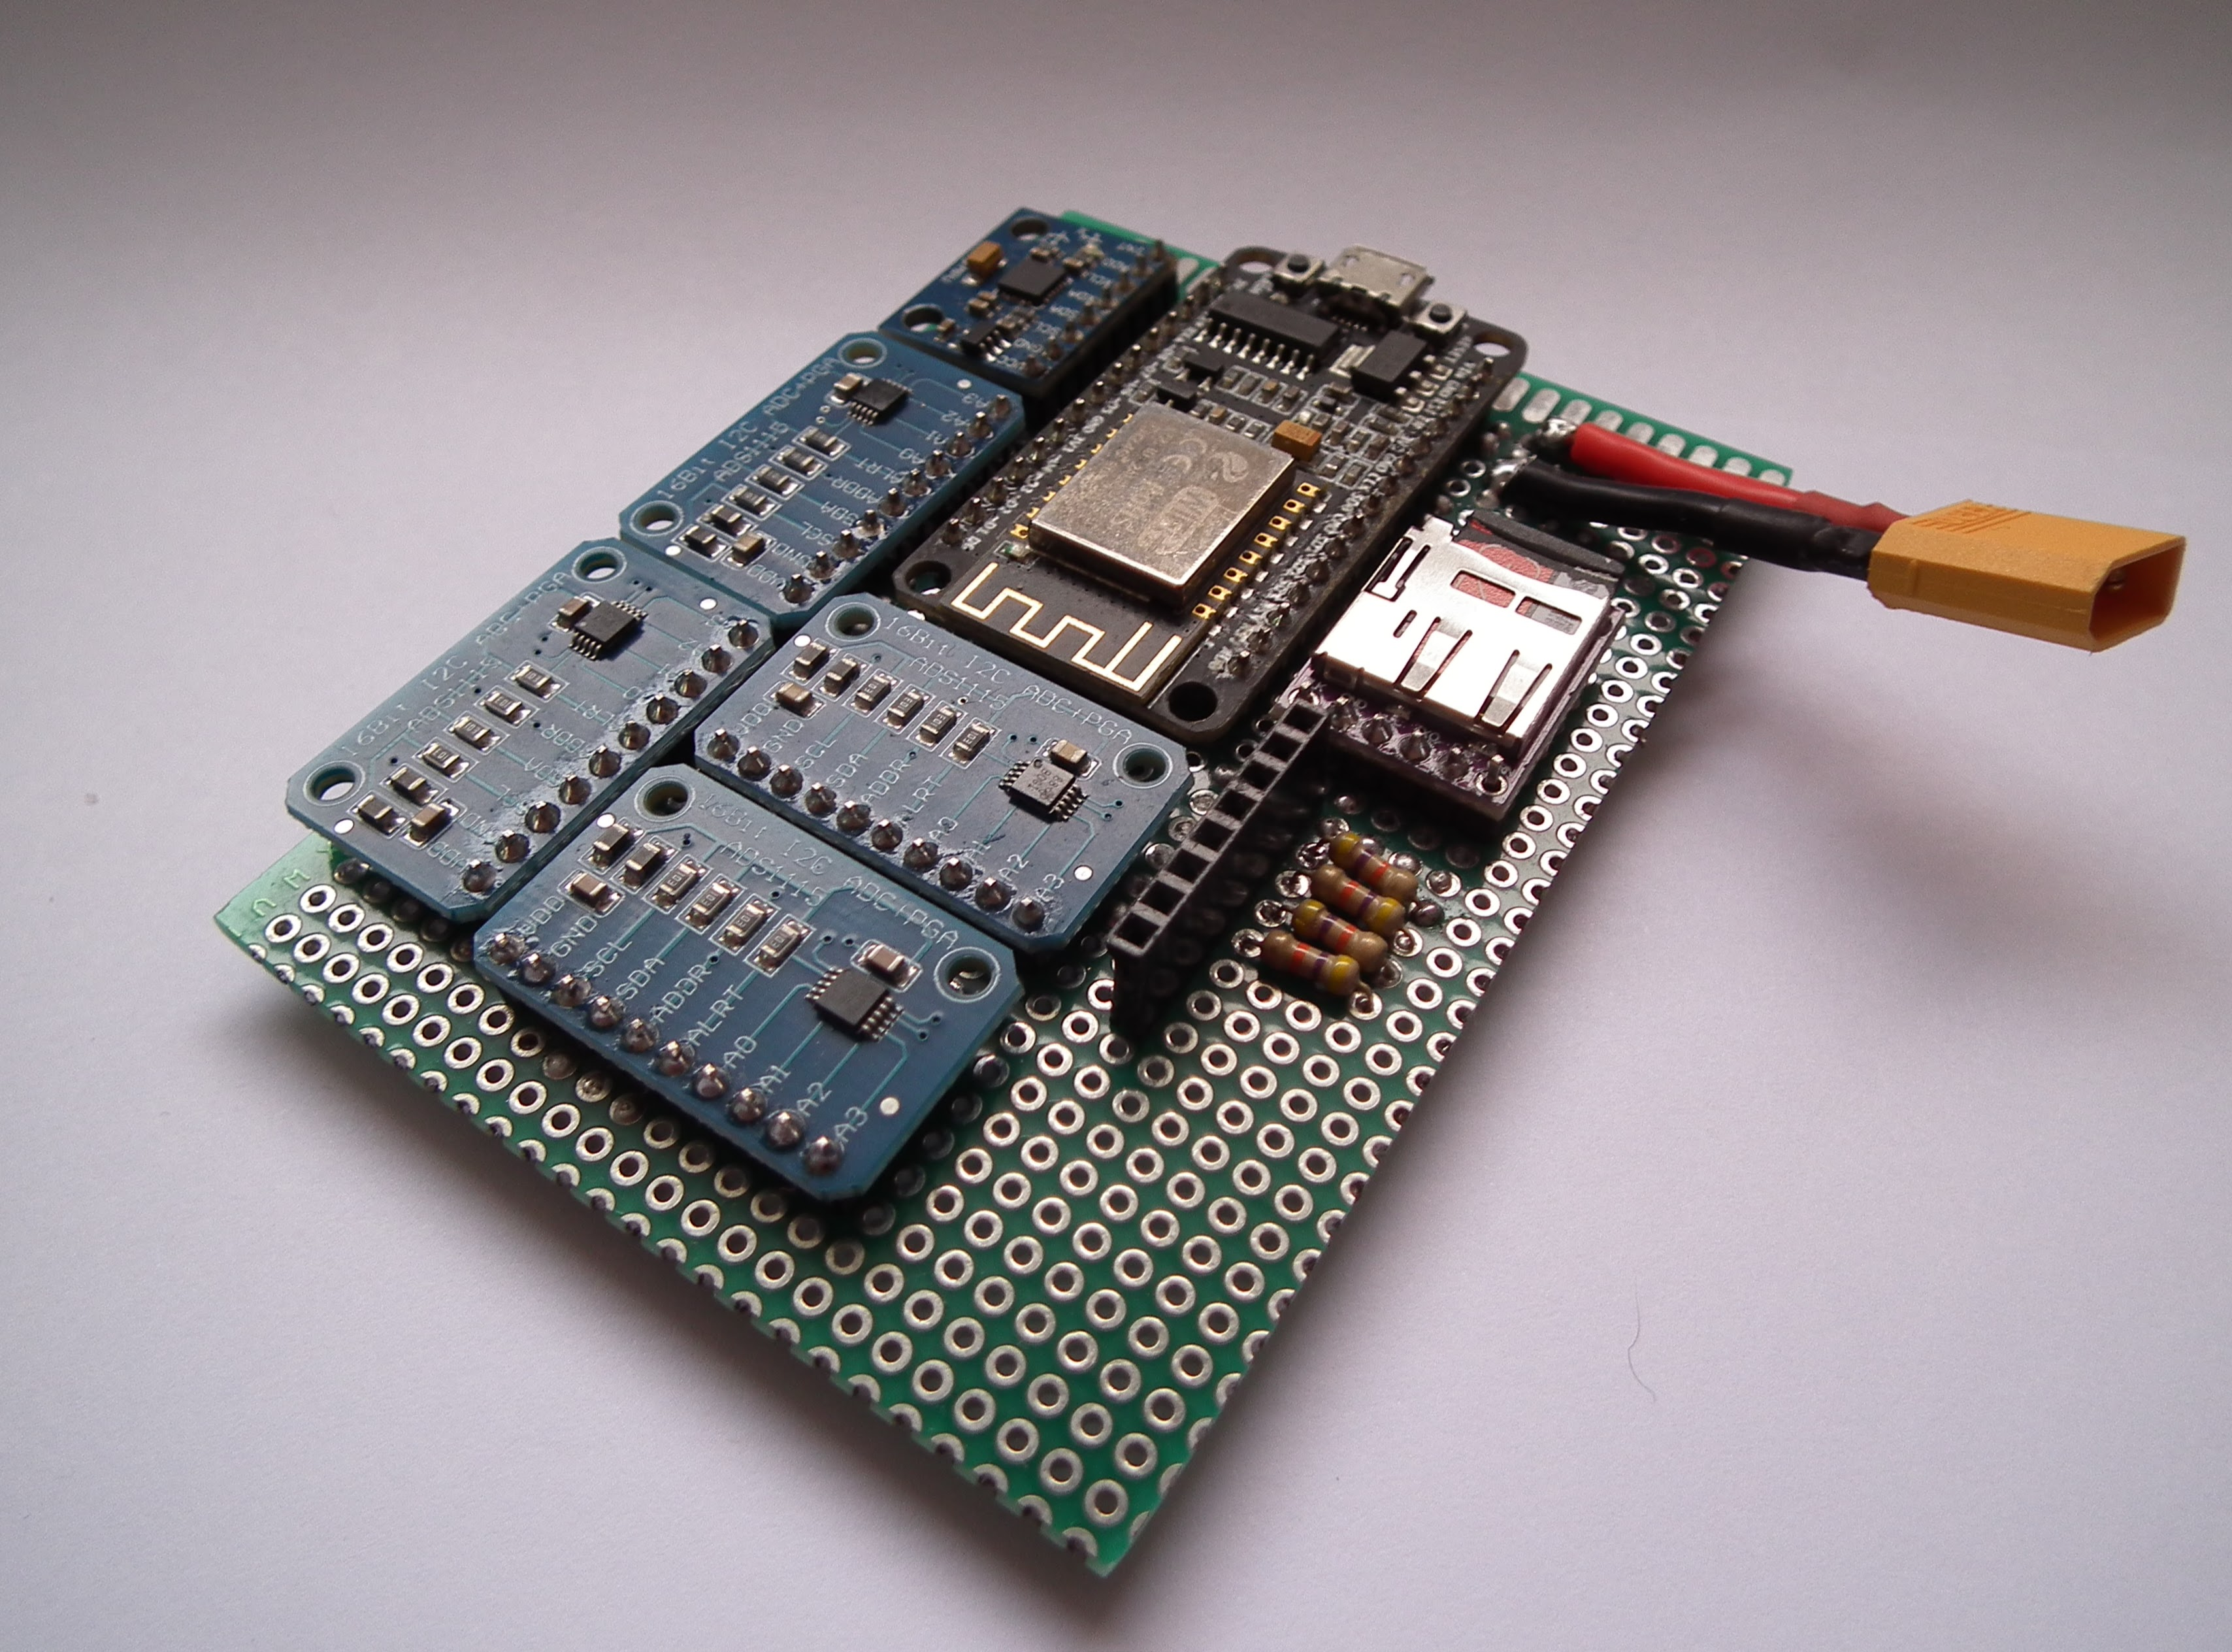
\includegraphics[width=\textwidth]{./figures/carte_00.jpg}

\end{frame}

\begin{frame}
    \frametitle{Le capteur de pression DF9-40}
    Le capteur de pression est une résistance variable de loi non linéaire.
    \begin{center}
        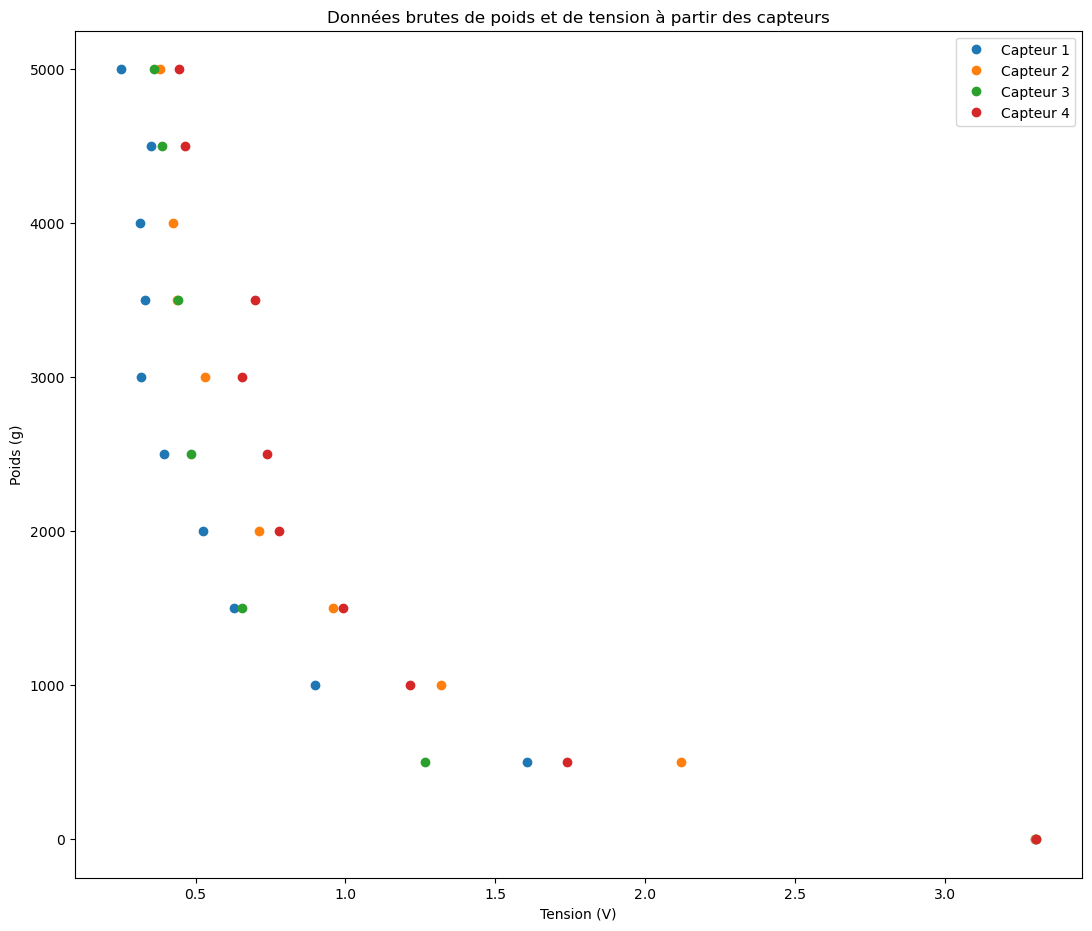
\includegraphics[scale=0.2]{./figures/cal_00.png}
    \end{center}
\end{frame}

\subsection{Calibration du dispositif}
\begin{frame}
    \frametitle{Calibration - ajustement de courbe 1/2}
    Envisageons la fonction suivante: $f_{a,b,c}(x) = \frac{a}{x^b}+c$\\
    \\
    Notons $x_i$ les valeurs en tension correspondant à un poids mesuré $y_i$.\\
    \\
    Il faut trouver a,b,c minimisant $ \sum_{i=0}^{n} (f_{a,b,c}(x_i)-y_i)^2$
\end{frame}

\begin{frame}
    \frametitle{Calibration - ajustement de courbe 2/2}
    Nous utilisons la méthode de la descente de gradient pour trouver une valeur approchée de a,b,c minimisant $C(a,b,c)=\sum_{i=0}^{n} (f_{a,b,c}(x_i)-y_i)^2$.
    \\
    \\
    L'ideal est d'avoir $\frac{\partial C}{\partial a} (a,b,c) = 0$ $\frac{\partial C}{\partial b} (a,b,c) = 0$ $\frac{\partial C}{\partial c} (a,b,c) = 0$, soit $\nabla C = 0$.
    \\
    \\
    Pour cela fixons $\alpha \in \mathbb{R}^+$, le taux d'apprentissage et un seuil $\varepsilon \in \mathbb{R}^+$.
    \\
    \\
    Nous construisons la suite $P_k=\begin{pmatrix} a_k \\ b_k \\ c_k \end{pmatrix}$ de la façon suivante:
    \begin{itemize}
        \item $P_0$ fixé de manière arbitraire
        \item $P_{k+1}= P_{k} - \alpha \times \nabla C$
    \end{itemize}
    Condition d'arrêt: $\nabla C < \varepsilon$
\end{frame}

\begin{frame}
    \frametitle{Calibration - résultats 1/2}
    Résultats de la méthode des moindres carrés avec la descente de gradient effectuée sur la carte:
    \begin{center}
        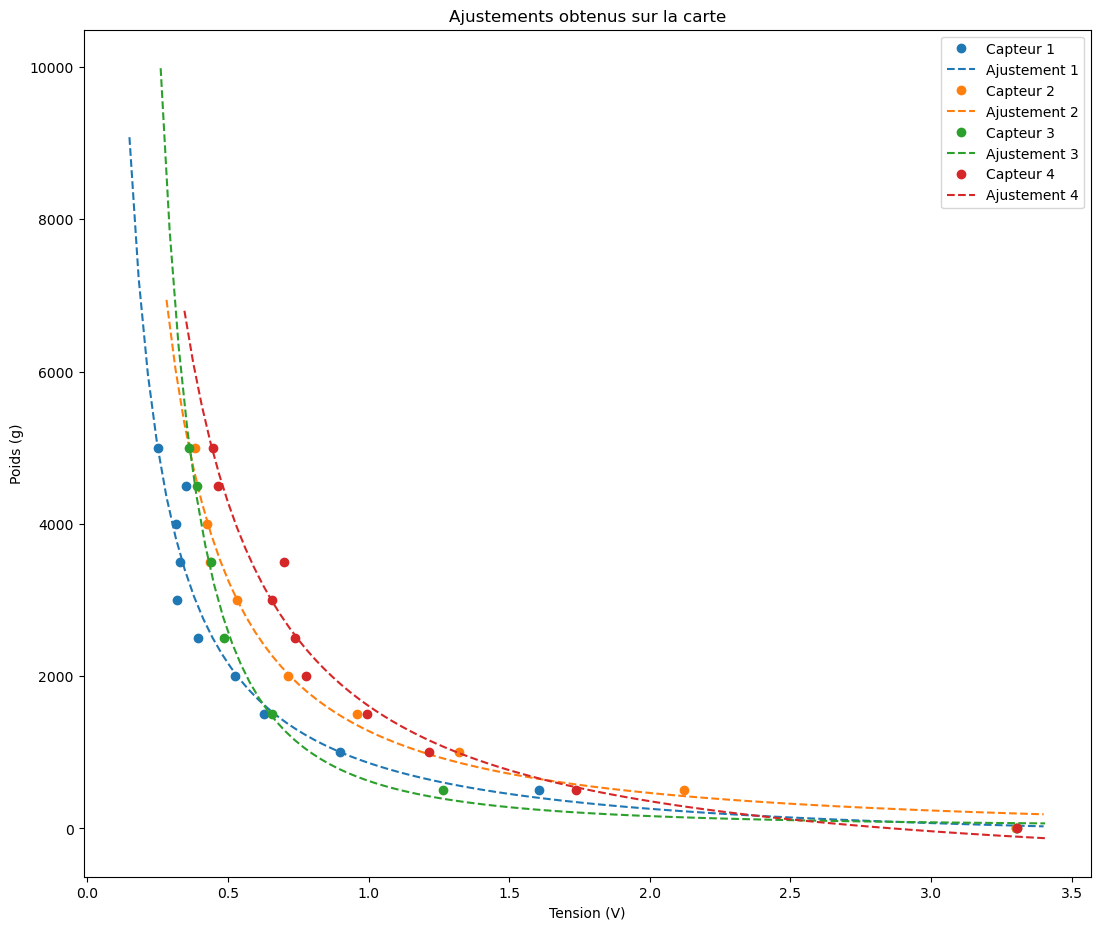
\includegraphics[scale=0.3]{./figures/cal_01.png}
    \end{center}
\end{frame}

\begin{frame}
    \frametitle{Calibration - résultats 2/2}
    Comparaison avec la fonction \texttt{curve\_fit} de \texttt{scipy}:
    \begin{center}
        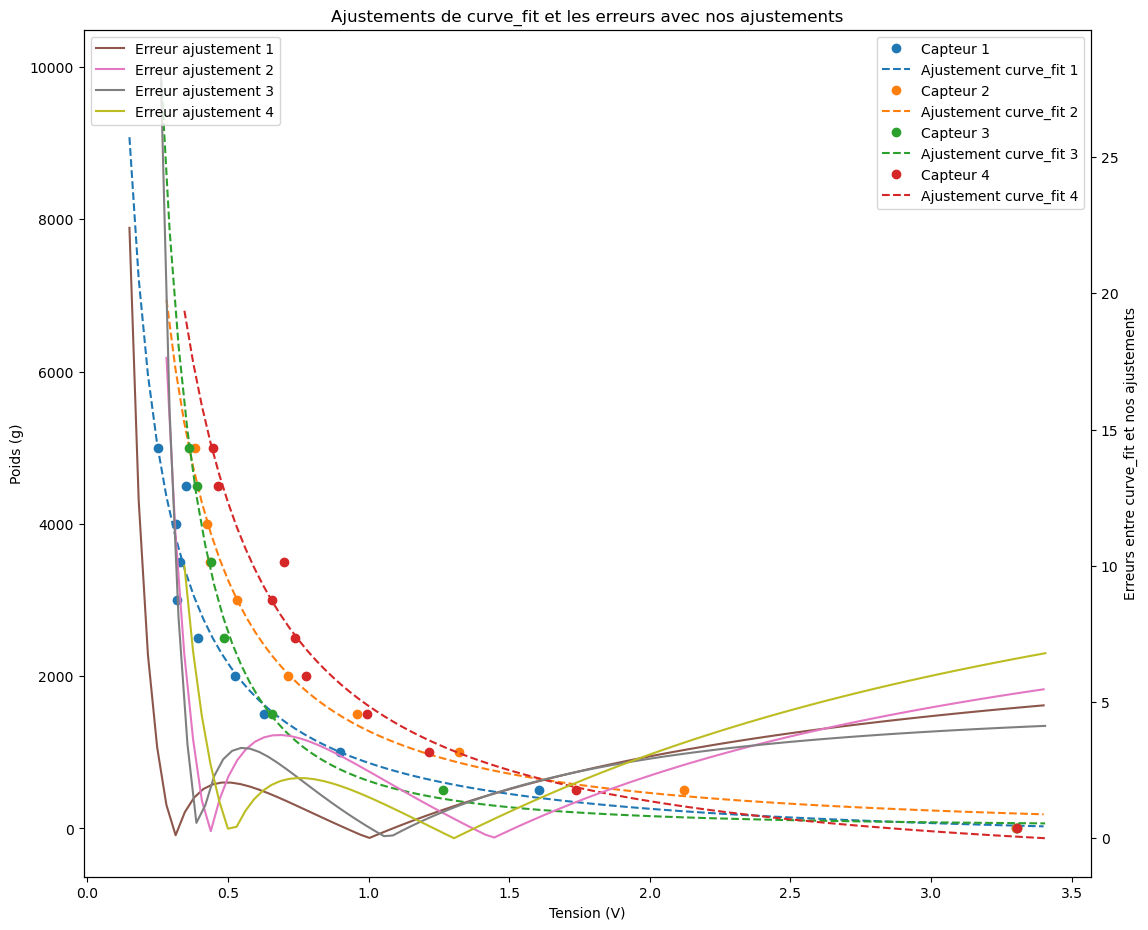
\includegraphics[scale=0.3]{./figures/cal_02.png}
    \end{center}
\end{frame}

\subsection{Premiers résultats}
\begin{frame}
    \frametitle{La semelle}
    Voici les capteurs disposés sur la semelle:
    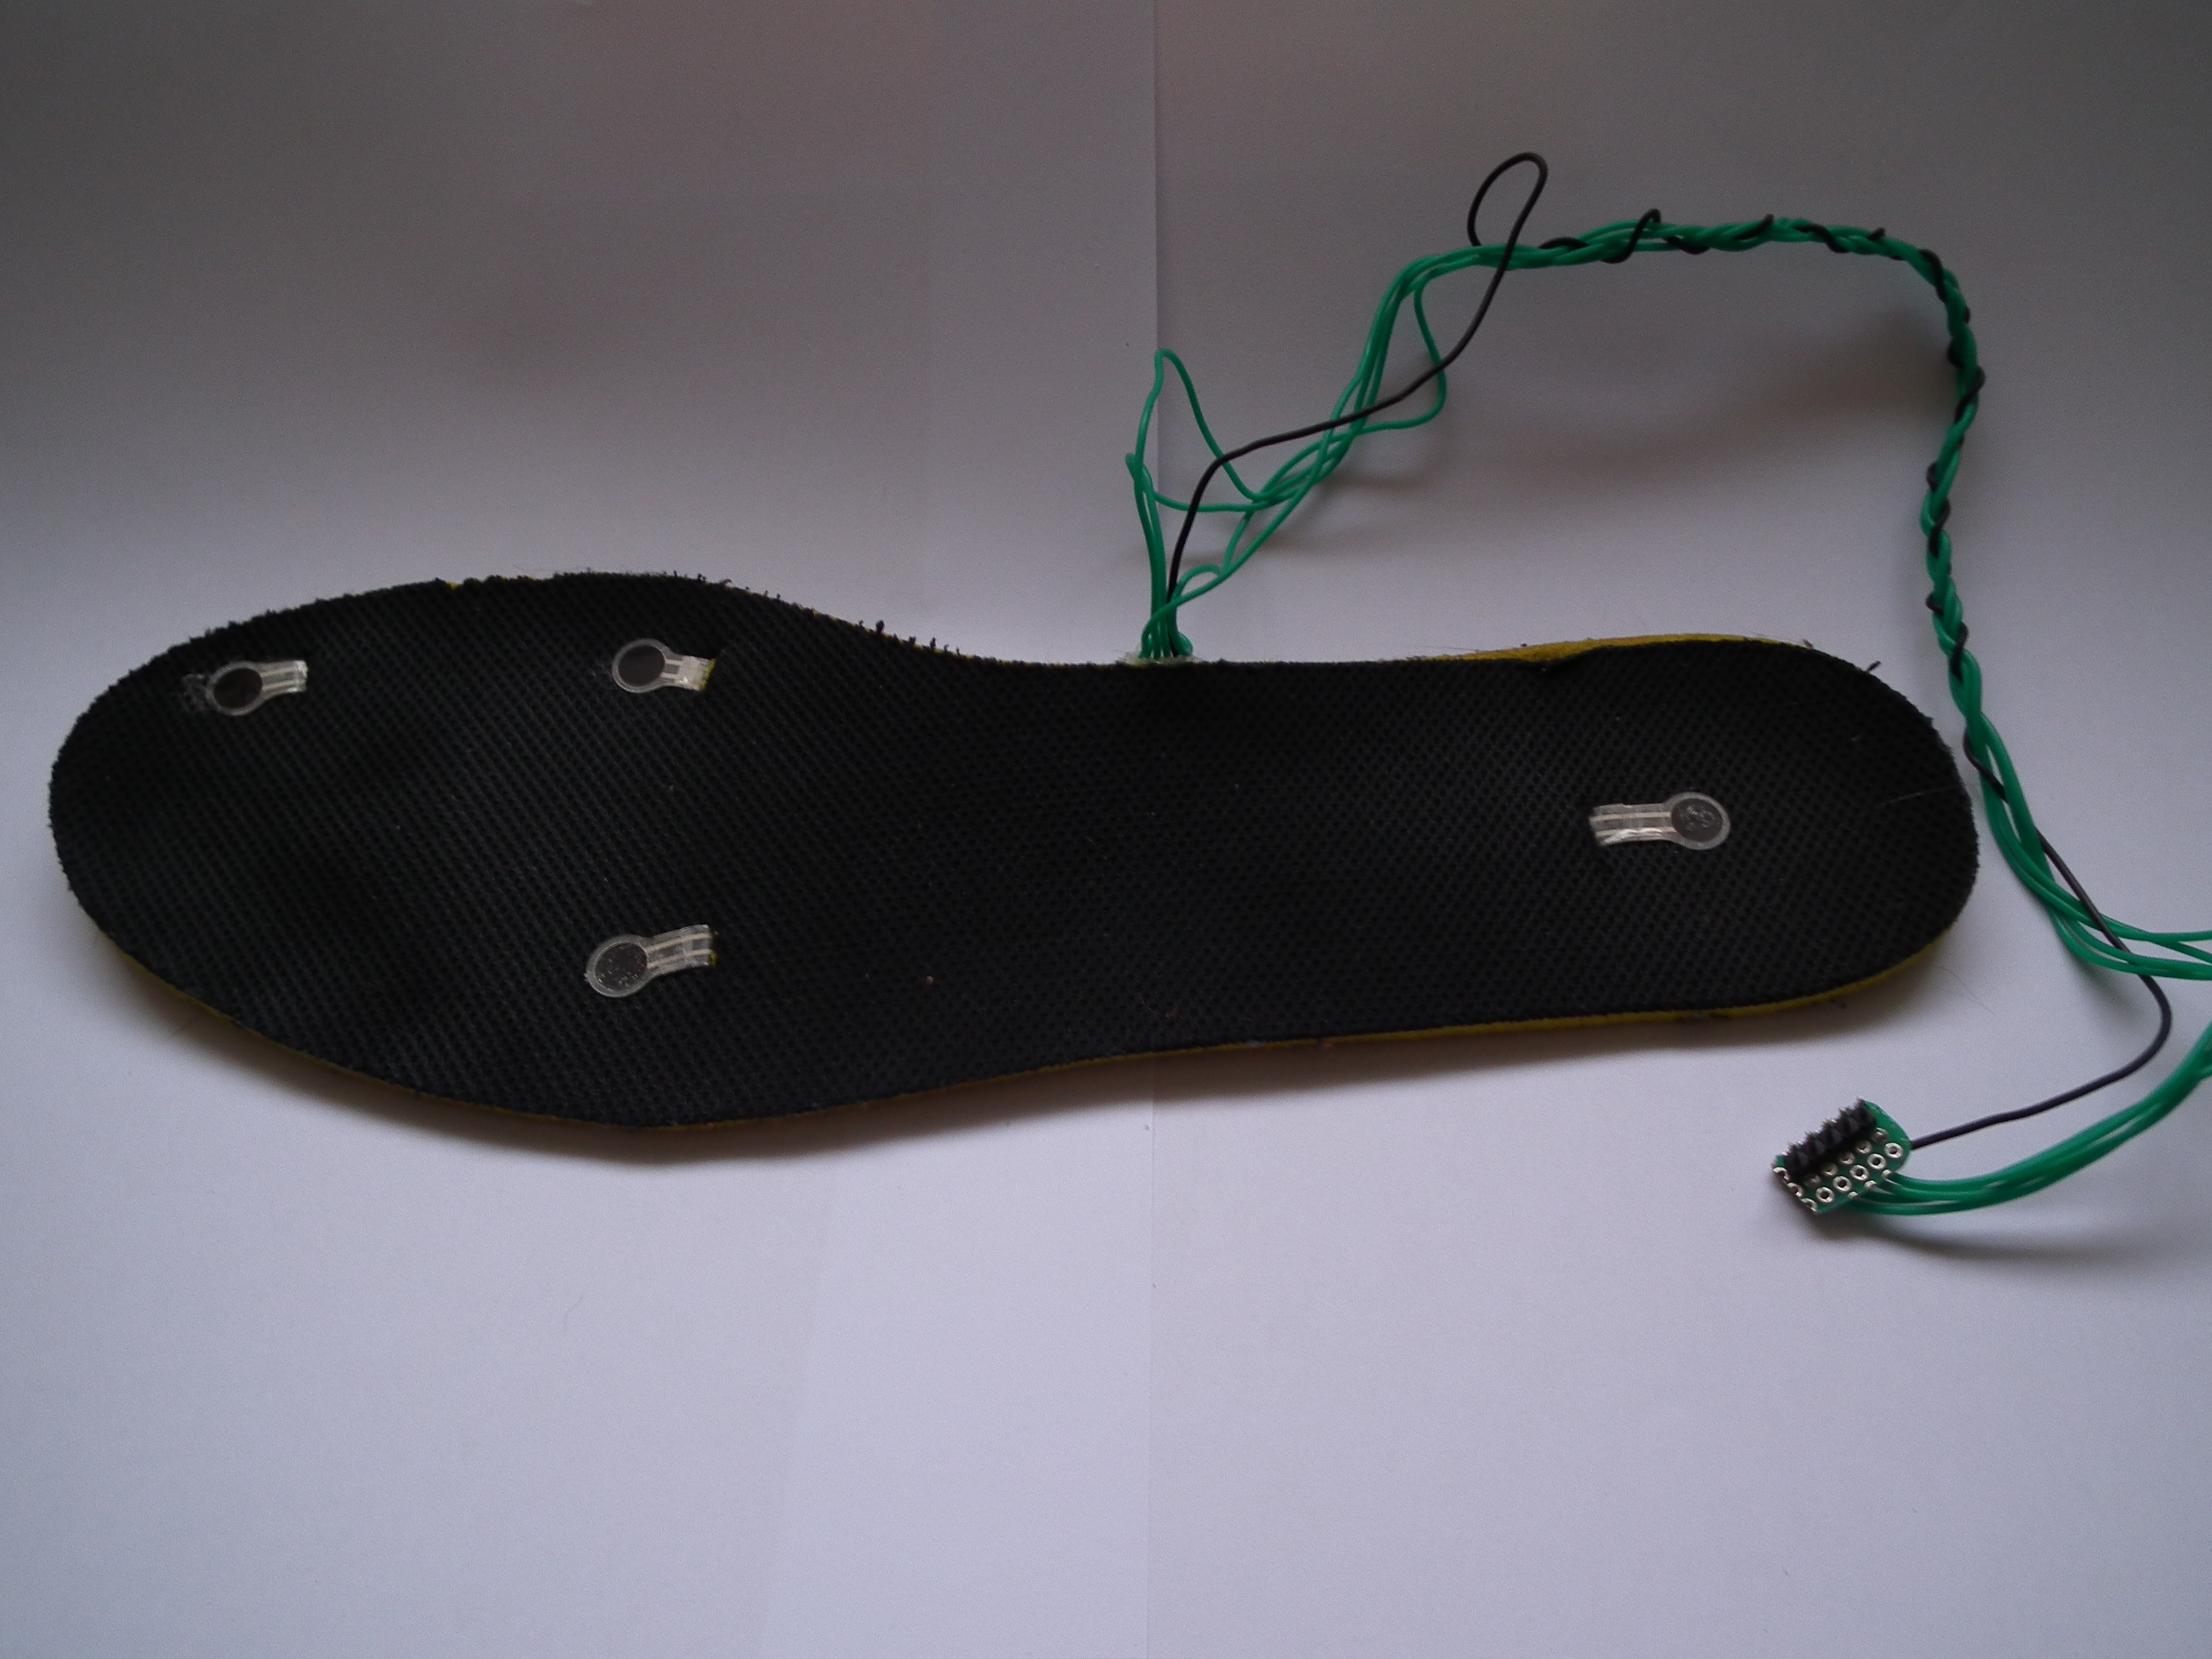
\includegraphics[width=\textwidth]{./figures/sem_00.jpg}

\end{frame}

\begin{frame}
    \frametitle{Les premiers résultats}
    Après avoir couru sur différents revêtements (béton, gravier, pelouse) avec des chaussures de ville et de course, nous obtenous:
    \begin{figure}
        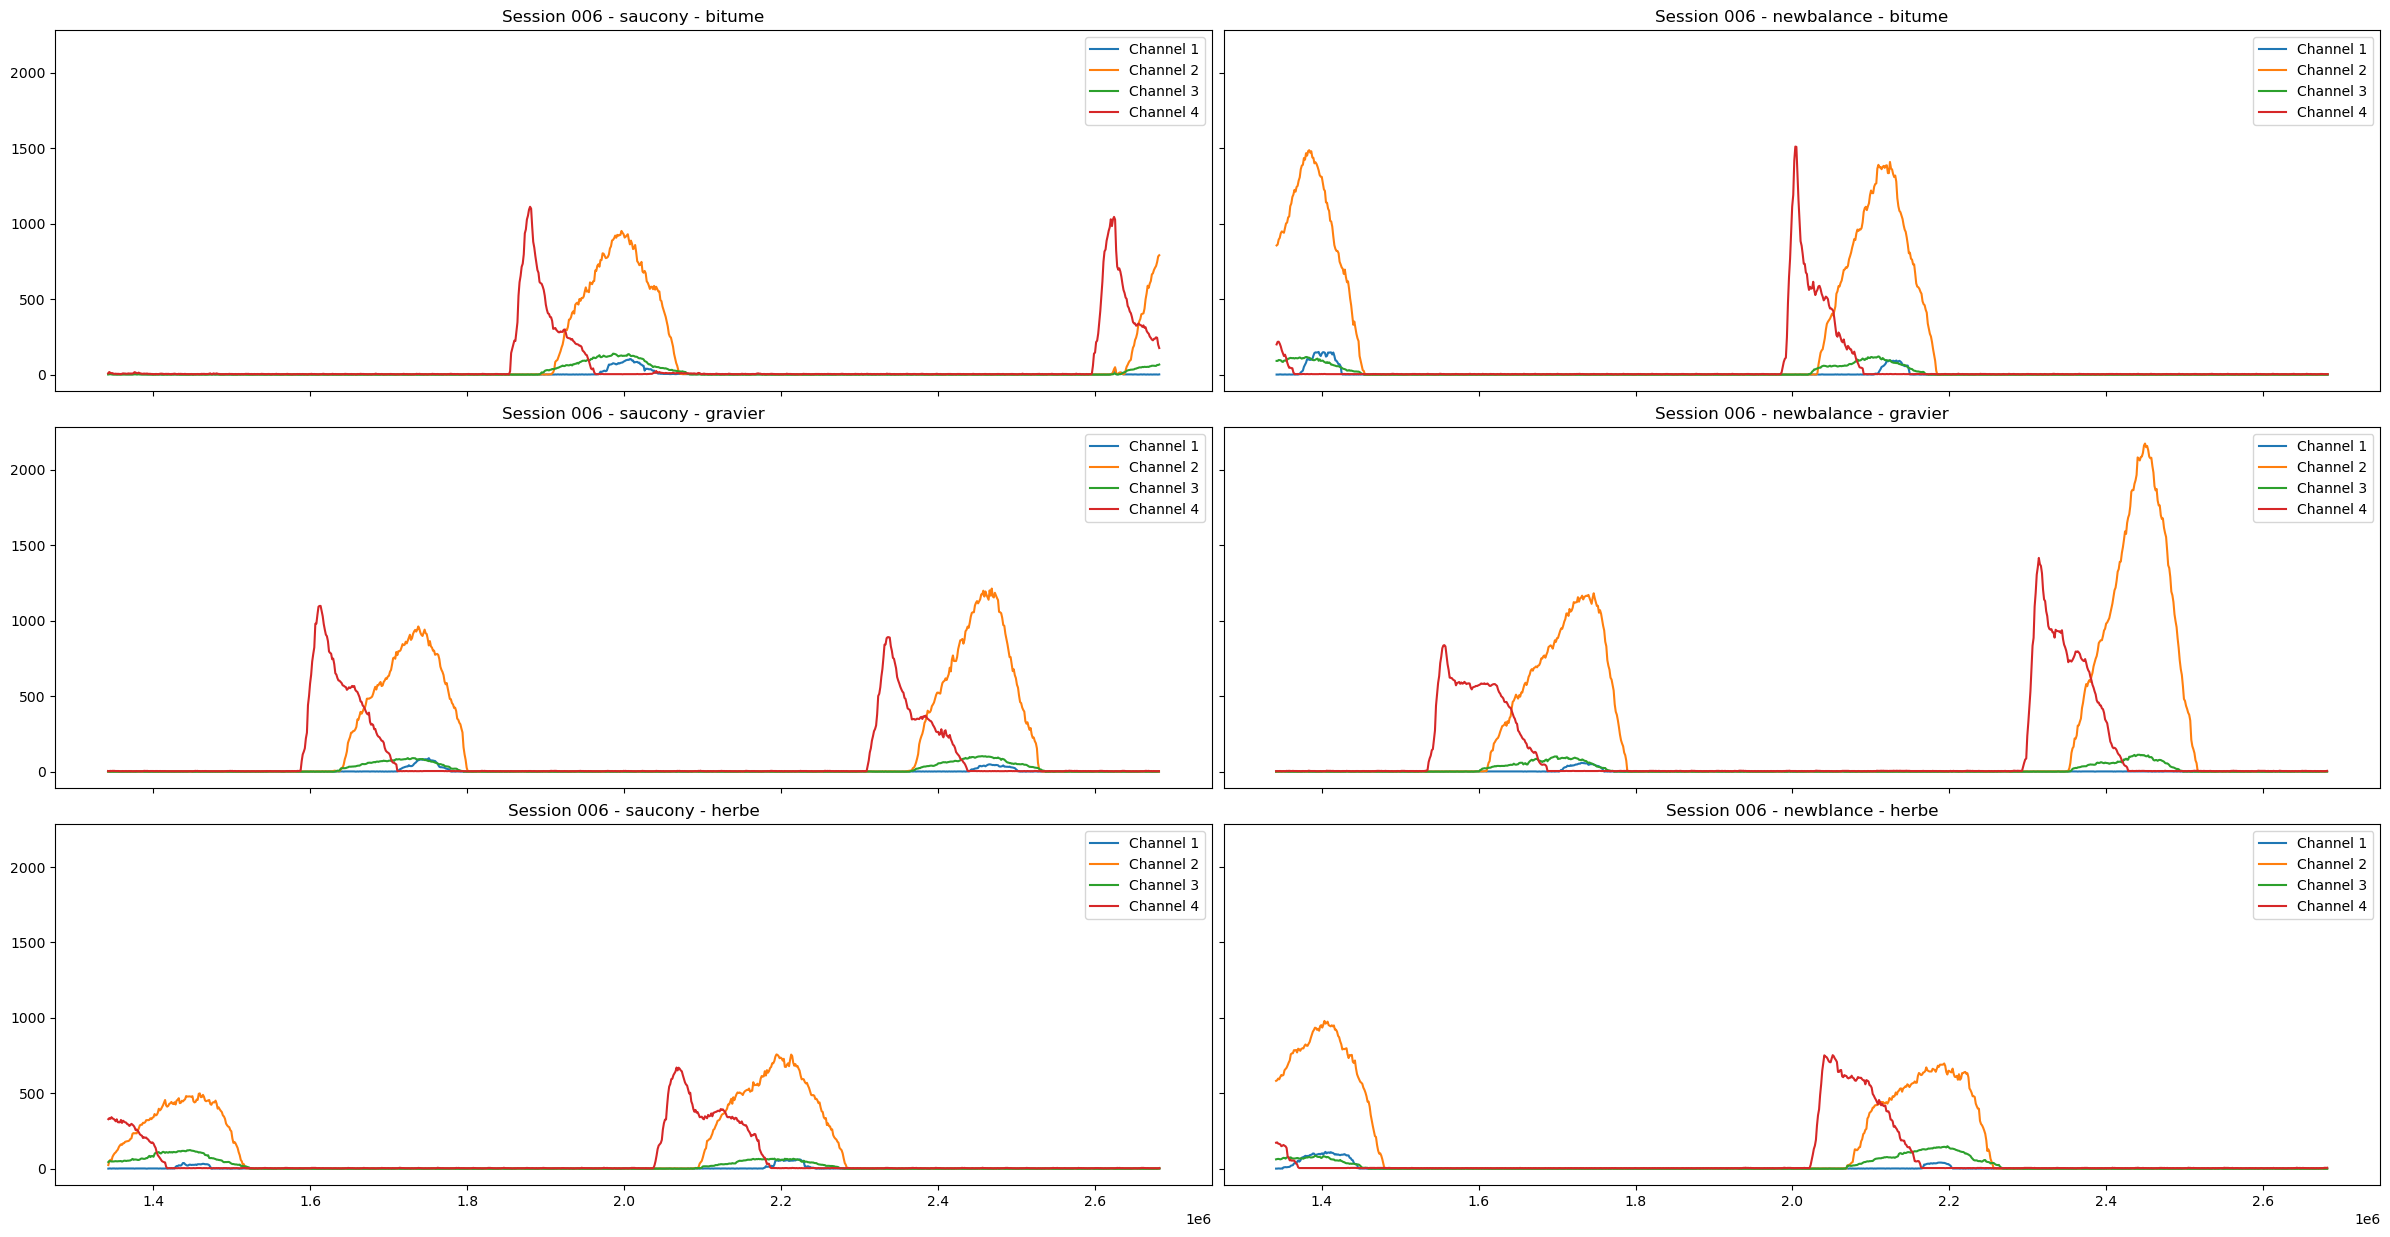
\includegraphics[scale=0.20]{./figures/res_01.png}
        \centering
    \end{figure}
\end{frame}
